\documentclass[english,reprint, aps, prl,superscriptaddress, showpacs,
showkeys, longbibliography, amsmath, amssymb, floatfix]{revtex4-1} 
\pdfoutput=1

\usepackage{fullpage}
\usepackage{cmap}
\usepackage[T1,T2A]{fontenc}
\usepackage[utf8]{inputenc}
\usepackage[french,main=english]{babel}
\usepackage{amsthm}
\usepackage{mathrsfs}
\usepackage{bbold}
\usepackage{wesa}
\usepackage{graphicx}
\usepackage{verbatim}
\usepackage[backref=false]{hyperref}
\usepackage{booktabs}
\usepackage{multirow}
\usepackage[braket,qm]{qcircuit}
\usepackage{color}
\usepackage[usenames,dvipsnames]{xcolor}
\usepackage{framed}
\usepackage{comment}
\usepackage{xparse}

\theoremstyle{plain}
\newtheorem{thm}{Theorem}
\newtheorem{lemma}{Lemma}[thm]
\newtheorem{cor}{Corollary}[thm]
\newtheorem{assumption}{Assumption}
\newtheorem{fact}{Fact}
\theoremstyle{definition}
\newtheorem{definition}{Definition}
\newtheorem{condition}[assumption]{Condition}
\setcounter{thm}{2}

\DeclareUnicodeCharacter{0229}{\c{e}}

\newcommand{\Hilb}{\mathcal{H}}
\newcommand{\events}{\ensuremath{\mathcal{E}}}
\newcommand{\qevents}{\ensuremath{\mathcal{E}}}
\newcommand{\pmeas}{\ensuremath{\mu}}
% \newcommand{\imposs}{{\text{\wesa{impossible}}}}
% \newcommand{\likely}{{\text{\wesa{likely}}}}
% \newcommand{\unlikely}{{\text{\wesa{unlikely}}}}
% \newcommand{\necess}{{\text{\wesa{certain}}}}
% \newcommand{\unknown}{{\text{\wesa{unknown}}}}
% \newcommand{\midd}{{\text{\wesa{middle}}}}
\newcommand{\imposs}{\ensuremath{\left[0,0\right]}}
\newcommand{\likely}{\ensuremath{\left[\tfrac{1}{2},1\right]}}
\newcommand{\unlikely}{\ensuremath{\left[0,\tfrac{1}{2}\right]}}
\newcommand{\necess}{\ensuremath{\left[1,1\right]}}
\newcommand{\unknown}{\ensuremath{\left[0,1\right]}}
\newcommand{\midd}{\ensuremath{\left[\tfrac{1}{4},\tfrac{3}{4}\right]}}
\newcommand{\fket}[1]{{|#1\rangle}}
\newcommand{\fproj}[1]{|#1\rangle\langle #1|}
\newcommand{\proj}[1]{\op{#1}{#1}}
\newcommand{\ps}{\texttt{+}}
\newcommand{\ms}{\texttt{-}}
\newcommand{\set}[2]{\ensuremath{\left\{ {#1}\mathrel{}\middle|\mathrel{}{#2}\right\} }}
\newcommand{\Tr}{\ensuremath{\mathop{\mathrm{Tr}}\nolimits}}
\allowdisplaybreaks
\newcommand{\coreBorn}{\ensuremath{\overline{\Hilb}}}
\newcommand{\mul}[1][]{\ensuremath{\mu^{L{#1}}}}
\newcommand{\mur}[1][]{\ensuremath{\mu^{R{#1}}}}
\setcounter{secnumdepth}{3}
% https://tex.stackexchange.com/questions/345284/can-i-have-an-almost-non-breaking-space-in-latex
% Change non-breaking space to \nolinebreak[1] 
% Hence, it will not hyphenate too much surrounding words.
\newcommand{\rmd}{d}
\newcommand{\rmi}{i}
\lineskiplimit=1pt
\newcommand{\ultramodular}{\mathcal{M}}
\newcommand{\ultramodularL}[1][]{\ensuremath{\ultramodular^{L{#1}}}}
\newcommand{\ultramodularR}[1][]{\ensuremath{\ultramodular^{R{#1}}}}
\newcommand{\muB}{\ensuremath{\mu^{B}}}
\newcommand{\eventsC}{\ensuremath{\events_{C}}}

\newcommand{\says}[3]{\begin{framed}\begin{minipage}{0.9\linewidth}\color{#1}{#2 says: #3}\end{minipage}\end{framed}}
\newcommand{\amr}[1]{\says{green}{Amr}{#1}}
\newcommand{\yutsung}[1]{\says{purple}{Yu-Tsung}{#1}}
\newcommand{\gerardo}[1]{\says{OliveGreen}{Gerardo}{#1}}
\newcommand{\andy}[1]{\says{blue}{Andy}{#1}}
% \excludecomment{suggest}
\NewDocumentEnvironment{suggest}{m m O{}}{#1{TEXT \##2 would go here. #3}}{#1{TEXT \##2 end here.}}

\newcommand{\happen}{\text{H}}
\newcommand{\notHappen}{\text{N}}
\newcommand{\missing}{?}

\begin{document}

\title{Response to the Referee Report for \\
``Quantum Interval-Valued Probability: Contextuality and the Born Rule''}
\date{\today}

\maketitle

%%%%%%%%%%%%%%%%%%%%%%%%%%%%%%%%%%%%%%%%%%%%%%%%%%%%%%%%%%%%%%%%%%%

In our QIVPM framework, the Kochen-Specker (KS) theorem is equivalent
to stating that there does not exist a ($\delta$=)$0$-deterministic
QIVPM. We further claim (Thm.~\ref{cor:Kochen-Specker-IVPM}) that
there cannot exist any $\delta$-deterministic QIVPM for
$\delta<\frac{1}{3}$ and that there exist QIVPMs for every
$\delta\ge\frac{1}{3}$.  The referee questions the correctness of
Thm.~\ref{cor:Kochen-Specker-IVPM} and the physical interpretation of
$\delta$-determinism. In answer to the question of correctness, we
attach, for the referee's convenience, an expanded complete proof of
Thm.~\ref{cor:Kochen-Specker-IVPM} at the end of this response. In the
next paragraphs, we explain the physical interpretation of
$\delta$-determinism and provide examples that illustrate why
$\frac{1}{3}$ is special.

%\bigskip 

\paragraph*{Experimental Data and $\delta$-determinism.} To the best of
our understanding, the argument against $\delta$-determinism by the
referee assumes that the parameter $\delta$ is \emph{exclusively}
related to the density of states defined in a general Hilbert
space. This is indeed Meyer's great insight and the main assumption in
his proof that using the field of rationals nullifies the KS theorem.
In other words, Meyer attributes finite-precision errors to the
description of the states, which is an idea that has been challenged
by several researchers, including Ax and Kochen (as cited by Cabello
2002), who argue that the effect of finite-precision measurements on
the KS theorem requires a different formalization. Our paper, indeed,
makes no particular assumptions about the description of the states,
and attributes finite-precision errors to the measurement process
itself as realized in a laboratory. In our framework, the parameter
$\delta$ reflects insufficient knowledge of the experimenter, which
could be due to a variety of reasons related to imperfections of
devices. A typical question that an experimenter may not be able to
answer accurately would be ``did an electron land in the left half or
the right half of the screen''? There are cases in which the electron
would land too close to the middle of the screen for the experimenter
to be able to determine with certainty that it was left or right of
the center. We simply record this imprecision in the probability we
assign to events, and use the axioms of probability theory
(additivity, convexity, etc) to argue that a sharp transition occurs
when the imprecision reaches a certain value. Our approach is agnostic
about attributing elements of reality to the state function (as
Meyer). We simply attribute lack of certainty to the measured results
through the use of an instrument.

To determine the probability of any event,
we typically repeat an experiment $n$ times and count the number
of times we witness the event. This assumes that for each run of the
experiment we can determine, using our apparatus, whether the event
occurred or not. Assume an event has an ideal mathematical probability
of $0$, and we repeat the experiment $100$ times. In a perfect world
we should be able to refute the event $100$ times and calculate that
the probability is $0$. We might also observe the event $2$ times
and refute it $98$ times and therefore calculate the probability
to be $0.02$. Note that this situation assumes perfect measurement
conditions.
%Let the quantum system be in state~$\ket{\psi}$ and the probability
%of some event  be $0$. Assume we repeat the experiment $100$ times
%and we observe the event $1$ time. The Godsil-Zaks-Meyer approach
%interprets this by assuming that the state was actually $\ket{\psi'}$
%which is infinitesimally close to $\ket{\psi}$ and proceed to reason
%about how coloring the states with rational points relates to the
%coloring of arbitrary states. We make no such assumptions and do not
%impose any constraints on the actual state of the system. In fact
%we do not make any statements about such situations. What we are addressing
%is a situation in which our devices do not allow to make a clear determination
%of whether an event has happened or not. We model this by an uncertainty
%in the probability of the event and then reason using the axioms of
%probability theory to bound this uncertainty. We should add that our
%approach is agnostic about attributing elements of reality to the
%state function (as Meyer). We simply attribute lack of certainty to
%the measured results through the use of an instrument. 
The question we focus on is what happens if we are only able to refute
it $97$ times and are \emph{uncertain} $3$ times? This is quite
common in actual experiments. Mathematically we can model this idea
by stating that the probability of the event is in the range $\left[0,0.03\right]$
which says that the probability of the event could be $0$, $0.01$,
$0.02$, or $0.03$ as each the three missing records could either
be evidence for the event or against it. We just cannot nail it down
given the current experimental results and therefore represent them as a ($\delta=$)$0.03$-deterministic
probability measure. The interesting observation is that the axioms
of probability theory (like additivity and convexity) impose enough
constraints on the structure of probability measures to make them
robust in the face of small $\delta$'s.

To see this in detail, consider a three-dimensional Hilbert space and
an experiment repeated $12$ times. By the KS theorem, it is impossible
to build a probability measure that maps every projection to either
$0=\frac{0}{12}$ or $1=\frac{12}{12}$. Now consider what happens if
$\frac{1}{4}$ of the data for every one-dimensional projector is
missing. A potential account of this degradation is to assign to each
event $P$ the entire range of possibilities $\bar{\mu}(P)$:
\begin{center}
\begin{tabular}{cc}
\toprule 
\addlinespace
$P$  & $\bar{\mu}\left(P\right)$\tabularnewline
\midrule
\midrule 
\addlinespace
$\mathbb{0}$ & $\imposs$\tabularnewline
\midrule 
\addlinespace
All one-dimensional projectors & $\left[0,\tfrac{1}{4}\right]$\tabularnewline
\midrule 
\addlinespace
All two-dimensional projectors & $\left[\tfrac{3}{4},1\right]$\tabularnewline
\midrule 
\addlinespace
$\mathbb{1}$ & $\necess$\tabularnewline
\bottomrule
\end{tabular}
\par\end{center}

\noindent This measure is not a valid QIVPM because it does not
satisfy the convexity condition: for any two orthogonal
one-dimensional events $P_{0}$ and $P_{1}$, the convexity condition
requires
$\bar{\mu}\left(P_{0}+P_{1}\right)\subseteq\bar{\mu}\left(P_{0}\right)+\bar{\mu}\left(P_{1}\right)$,
but $\bar{\mu}\left(P_{0}+P_{1}\right)=\left[\tfrac{3}{4},1\right]$
which is not a subset of
$\left[0,\tfrac{1}{2}\right]=\bar{\mu}\left(P_{0}\right)+\bar{\mu}\left(P_{1}\right)$. Interestingly,
it is impossible to find any probability measure that would be
consistent with these observations as the interval
$\left[\tfrac{3}{4},1\right]$ is completely disjoint from the interval
$\left[0,\tfrac{1}{2}\right]$ and no amount of shifting of assumptions
regarding the precise outcome of the missing observations could change
that disjointness. However, a sharp transition occurs when
$\delta=\tfrac{1}{3}$ as shown next. 

%% Indeed for every one-dimensional projector, the missing
%% data could either refute or support the associated event. 
%% This yields the following probability measure~$\bar{\mu}$
%% as a possible formalization, where the column labeled by $P$ lists
%% projectors, and the column labeled by $\bar{\mu}\left(P\right)$ lists
%% the probability of these projectors.

In case the missing data reaches $\frac{1}{3}$, the probability
measure that assigns to each event the entire range of possibilities
is:
\begin{center}
\begin{tabular}{cc}
\toprule 
\addlinespace
$P$  & $\bar{\mu}\left(P\right)$\tabularnewline
\midrule
\midrule 
\addlinespace
$\mathbb{0}$ & $\imposs$\tabularnewline
\midrule 
\addlinespace
All one-dimensional projectors & $\left[0,\tfrac{1}{3}\right]$\tabularnewline
\midrule 
\addlinespace
All two-dimensional projectors & $\left[\tfrac{2}{3},1\right]$\tabularnewline
\midrule 
\addlinespace
$\mathbb{1}$ & $\necess$\tabularnewline
\bottomrule
\end{tabular}
\par\end{center}

\noindent This is also not a valid probability measure by the same
argument as above. However, in this case
$\bar{\mu}\left(P_{0}+P_{1}\right)=\left[\tfrac{2}{3},1\right]$ and
$\left[0,\tfrac{2}{3}\right]=\bar{\mu}\left(P_{0}\right)+\bar{\mu}\left(P_{1}\right)$
have a common point. And hence by assuming that the missing data for
one-dimensional projectors always support the associated event, while
those for two-dimensional projectors always refute the event, we can
find the following probability measure which can verified to be a
valid QIVPM and which is consistent with the experimental data:
\begin{center}
\begin{tabular}{cc}
\toprule 
\addlinespace
$P$  & $\bar{\mu}\left(P\right)$\tabularnewline
\midrule
\midrule 
\addlinespace
$\mathbb{0}$ & $\imposs$\tabularnewline
\midrule 
\addlinespace
All one-dimensional projectors & $\left[\tfrac{1}{3},\tfrac{1}{3}\right]$\tabularnewline
\midrule 
\addlinespace
All two-dimensional projectors & $\left[\tfrac{2}{3},\tfrac{2}{3}\right]$\tabularnewline
\midrule 
\addlinespace
$\mathbb{1}$ & $\necess$\tabularnewline
\bottomrule
\end{tabular}
\par\end{center}

A similar situation happens when more than $\frac{1}{3}$ of data is
missing. In particular, having half of the data missing, the
probability measure that assigns to each event the entire range of
possibilities is already a QIVPM:

\begin{center}
\begin{tabular}{cc}
\toprule 
\addlinespace
$P$  & $\bar{\mu}\left(P\right)$\tabularnewline
\midrule
\midrule 
\addlinespace
$\mathbb{0}$ & $\imposs$\tabularnewline
\midrule 
\addlinespace
All one-dimensional projectors & $\left[0,\tfrac{1}{2}\right]$\tabularnewline
\midrule 
\addlinespace
All two-dimensional projectors & $\left[\tfrac{1}{2},1\right]$\tabularnewline
\midrule 
\addlinespace
$\mathbb{1}$ & $\necess$\tabularnewline
\bottomrule
\end{tabular}
\par\end{center}

The above arguments could be summarized and illustrated using the following figure: 
\begin{center}
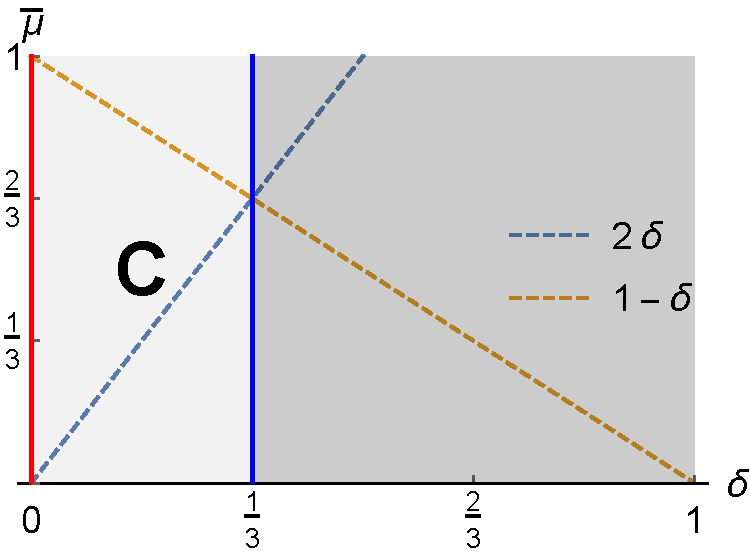
\includegraphics[scale=0.5]{prop_letter_ajhs_referee_response_nb}
\par\end{center}

\noindent The region to the left of the vertical line at
$\delta=\frac{1}{3}$ is where we assume small measurement degradation;
in that region our extension of the KS theorem definitely demonstrates
contextuality ({\bf{\sf C}}). In the region to the right, the degradation of the data
is large and our extension of the KS theorem no longer refutes other
explanations for the experimental data.

\bigskip

\paragraph*{Mermin-Peres ``Magic Square''.} We now use this same idea
to analyze the Mermin-Peres ``magic square'' argument. We show that
when the measurements are infinitely precise, the Mermin-Peres ``magic
square'' argument definitely demonstrates contextuality. But as we
progressively degrade the certainty of the data, a transition happens
in which the Mermin-Peres ``magic square'' argument no longer
demonstrates contextuality. Consider the nine observables
$\mathbf{O}_{ij}$ with $i$ and $j$ ranging over $\{0,1,2\}$,
corresponding to the Mermin-Peres ``magic square'' used to illustrate the
KS theorem:

{\renewcommand{\arraystretch}{2}% 
\begin{center} 
\begin{tabular}{r|@{\quad}c@{\quad}|@{\quad}c@{\quad}|@{\quad}c@{\quad}|} 
$\mathbf{O}_{ij}$~ & $j=0$ & $j=1$ & $j=2$ \\ 
\hline  
$i=0~$ & $\mathbb{1}\otimes\sigma_{z}$  & $\sigma_{z}\otimes\mathbb{1}$  & $\sigma_{z}\otimes\sigma_{z}$ \tabularnewline 
\hline  
$i=1~$ & $\sigma_{x}\otimes\mathbb{1}$  & $\mathbb{1}\otimes\sigma_{x}$  & $\sigma_{x}\otimes\sigma_{x}$ \tabularnewline 
\hline  
$i=2~$ & $\sigma_{x}\otimes\sigma_{z}$  & $\sigma_{z}\otimes\sigma_{x}$  & $\sigma_{y}\otimes\sigma_{y}$ \tabularnewline 
\hline  
\end{tabular}\,.
\par\end{center} 
}

\noindent The observables are constructed using the Pauli matrices
$\left\{ \mathbb{1},\sigma_{x},\sigma_{y},\sigma_{z}\right\} $ whose
eigenvalues are all either~$1$ or $-1$.
They are arranged such that in each row and column, \emph{except the
column $j=2$}, every observable and its expectation value is the
product of the other two. In the $j=2$ column, we have instead that
$\left(\sigma_{z}\otimes\sigma_{z}\right)\left(\sigma_{x}\otimes\sigma_{x}\right)=-\sigma_{y}\otimes\sigma_{y}$
and 
\begin{equation}
\expval{\mathbf{O}_{02}}\expval{\mathbf{O}_{12}}=-\expval{\mathbf{O}_{22}}\,.\label{eq:j_2_expectation_value}
\end{equation}

Assume we measure each observable twice. By the KS theorem, it is
impossible to get the following measurement results because the product
of the expectation values in the $j=2$ column violates Eq.~(\ref{eq:j_2_expectation_value}).
\begin{center}
\begin{tabular}{cccc}
\toprule 
\addlinespace
$\mathbf{O}_{ij}$  & \multicolumn{2}{c}{Results} & $\begin{aligned} & \textrm{Possible}\\
 & \expval{\mathbf{O}_{ij}}
\end{aligned}
$\tabularnewline
\midrule
\midrule 
\addlinespace
$\mathbf{O}_{00}$, $\mathbf{O}_{11}$ & $-1$ & $-1$ & $-1$\tabularnewline
\midrule 
\addlinespace
$\mathbf{O}_{01}$ , $\mathbf{O}_{10}$  & $-1$ & $-1$ & $-1$\tabularnewline
\midrule 
\addlinespace
$\mathbf{O}_{02}$ , $\mathbf{O}_{12}$ & $1$ & $1$ & $1$\tabularnewline
\midrule 
\addlinespace
$\mathbf{O}_{20}$ , $\mathbf{O}_{22}$ , $\mathbf{O}_{21}$  & $1$ & $1$ & $1$\tabularnewline
\bottomrule
\end{tabular}
\par\end{center}

Now consider what happens if half of the records are missing, i.e.,
$\delta=\frac{1}{2}$, which gives the following measurement results,
where $\missing$ stands for missing data.
\begin{center}
\begin{tabular}{ccccc}
\toprule 
\addlinespace
$\mathbf{O}_{ij}$  & \multicolumn{2}{c}{Results} & $\begin{aligned} & \textrm{Missing}\\
 & \textrm{Record}\\
 & \textrm{Might Be}
\end{aligned}
$ & $\begin{aligned} & \textrm{Possible}\\
 & \expval{\mathbf{O}_{ij}}
\end{aligned}
$\tabularnewline
\midrule
\midrule 
\addlinespace
$\mathbf{O}_{00}$, $\mathbf{O}_{11}$ & $-1$ & $\missing$ & $1$ & $0$\tabularnewline
\midrule 
\addlinespace
$\mathbf{O}_{01}$ , $\mathbf{O}_{10}$  & $\missing$ & $-1$ & $1$ & $0$\tabularnewline
\midrule 
\addlinespace
$\mathbf{O}_{02}$ , $\mathbf{O}_{12}$ & $1$ & $\missing$ & $-1$ & $0$\tabularnewline
\midrule 
\addlinespace
$\mathbf{O}_{20}$ , $\mathbf{O}_{22}$ , $\mathbf{O}_{21}$  & $\missing$ & $1$ & $-1$ & $0$\tabularnewline
\bottomrule
\end{tabular}
\par\end{center}

\noindent Since the experimental results are missing, they might come
from the third column. In this situation, the expectation values of
each observables is always $0$, and the product relations among these
expectation values is consistent with the product relations among
observables. 

\bigskip 

\paragraph*{Expanded Proof of Thm.~3.}

\begin{thm}[Finite-precision Extension of the Kochen-Specker Theorem]
\label{cor:Kochen-Specker-IVPM} Given a Hilbert space $\Hilb$ of
dimension~$d\ge3$, there is no $\delta$-deterministic QIVPM for
$\delta<\frac{1}{3}$.\end{thm}

The proof is by contradiction: Suppose there is a $\delta$-deterministic
QIVPM~$\bar{\mu}:\events\rightarrow\mathscr{I}$. Now use this assumed
QIVPM to construct the following $0$-deterministic QIVPM $\bar{\mu}^{\textrm{D}}:\events\rightarrow\left\{ \imposs,\necess\right\} $:
\begin{equation}
\bar{\mu}^{\textrm{D}}\left(P\right)=\begin{cases}
\imposs\,, & \textrm{ if }\bar{\mu}\left(P\right)\subseteq\left[0,\delta\right]\:;\\
\necess\,, & \textrm{ if }\bar{\mu}\left(P\right)\subseteq\left[1-\delta,1\right]\:.
\end{cases}
\end{equation}
However, since we know that $0$-deterministic QIVPMs do not exist,
the map $\bar{\mu}^{\textrm{D}}$ cannot exist and hence $\bar{\mu}$
does not exist. It remains to verify that $\bar{\mu}^{\textrm{D}}$
is indeed a QIVPM by checking that for orthogonal projectors $P_{0}$
and~$P_{1}$, 
\begin{equation}
\bar{\mu}^{\textrm{D}}\left(P_{0}+P_{1}\right)=\bar{\mu}^{\textrm{D}}\left(P_{0}\right)+\bar{\mu}^{\textrm{D}}\left(P_{1}\right)\,,\label{eq:QuantumInterval-valuedProbability-Equal}
\end{equation}
because Eq.~(\ref{eq:QuantumInterval-valuedProbability-Equal}) implies
the convexity condition.

When one of $\bar{\mu}^{\textrm{D}}\left(P_{0}\right)$ and $\bar{\mu}^{\textrm{D}}\left(P_{1}\right)$
is $\necess$, say $\bar{\mu}^{\textrm{D}}\left(P_{0}\right)=\necess$
and $\bar{\mu}^{\textrm{D}}\left(P_{1}\right)=\imposs$, we have $\bar{\mu}\left(P_{0}\right)\subseteq\left[1-\delta,1\right]$
and $\bar{\mu}\left(P_{1}\right)\subseteq\left[0,\delta\right]$ which
implies $\bar{\mu}\left(P_{0}+P_{1}\right)\subseteq\left[1-\delta,1+\delta\right]$.
Since $\bar{\mu}\left(P_{0}+P_{1}\right)$ is a subset of $\left[0,1\right]$,
$\bar{\mu}\left(P_{0}+P_{1}\right)$ must be a subset of $\left[1-\delta,1\right]$,
which implies $\bar{\mu}^{\textrm{D}}\left(P_{0}+P_{1}\right)=\necess$.

When
$\bar{\mu}^{\textrm{D}}\left(P_{0}\right)=\bar{\mu}^{\textrm{D}}\left(P_{1}\right)=\imposs$,
we have both $\bar{\mu}\left(P_{0}\right)$ and
$\bar{\mu}\left(P_{1}\right)\subseteq\left[0,\delta\right]$ which
implies
$\bar{\mu}\left(P_{0}+P_{1}\right)\subseteq\left[0,2\delta\right]$.
Since $\delta<\frac{1}{3}$, $\left[0,2\delta\right]$ and
$\left[1-\delta,1\right]$ are disjoint, which implies
$\bar{\mu}\left(P_{0}+P_{1}\right)$ and $\left[1-\delta,1\right]$ are
disjoint. Together with the fact that
$\bar{\mu}\left(P_{0}+P_{1}\right)$ is a subset of either
$\left[0,\delta\right]$ or $\left[1-\delta,1\right]$,
$\bar{\mu}\left(P_{0}+P_{1}\right)$ must be a subset of
$\left[0,\delta\right]$, which implies
$\bar{\mu}^{\textrm{D}}\left(P_{0}+P_{1}\right)=\imposs$.
\end{document}

